%======================================================
% CHAPTER III: SWR - SOFTWARE REQUIREMENTS SPECIFICATION
%======================================================
\chapter{SWR -- ĐẶC TẢ YÊU CẦU PHẦN MỀM}

\section{Tổng quan Tài liệu SWR}

Tài liệu \textbf{Đặc tả Yêu cầu Phần mềm (Software Requirements Specification -- SWR)} mô tả đầy đủ và chi tiết các yêu cầu đối với hệ thống Chatbot hỗ trợ học tập ứng dụng RAG. Tài liệu này là cơ sở cốt lõi để nhóm phát triển tiến hành thiết kế kiến trúc, lập trình, kiểm thử và đánh giá mức độ hoàn thiện của hệ thống.

\begin{table}[H]
  \centering
  \caption{Thông tin tài liệu SWR}
  \label{tab:swr-info}
  \renewcommand{\arraystretch}{1.4}
  \begin{tabularx}{\textwidth}{|l|X|}
    \hline
    \rowcolor{blue!10}
    \textbf{Mục} & \textbf{Nội dung} \\
    \hline
    Phiên bản & 1.0 \\
    \hline
    Ngày tạo & 07/2026 \\
    \hline
    Đối tượng áp dụng & Đội phát triển, giảng viên, khách hàng \\
    \hline
    Phạm vi & Hệ thống Chatbot RAG -- Nhóm 9 \\
    \hline
  \end{tabularx}
\end{table}

%------------------------------------------------------
\section{Tổng quan Sản phẩm (Product Overview)}
%------------------------------------------------------

\subsection{Biểu đồ Ngữ cảnh (Context Diagram)}

Biểu đồ Context mô tả hệ thống ở mức độ trừu tượng cao nhất, thể hiện các tác nhân bên ngoài và các luồng dữ liệu chính trao đổi với hệ thống Chatbot.

\begin{figure}[H]
  \centering
  
\includegraphics[width=0.95\textwidth]{images/context.png}
  \caption{Biểu đồ Ngữ cảnh (Context Diagram) của hệ thống}
  \label{fig:context}
\end{figure}

Trong biểu đồ Context, hệ thống Chatbot (Backend FastAPI) đóng vai trò trung tâm:
\begin{itemize}[itemsep=3pt]
  \item \textbf{Sinh viên} $\leftrightarrow$ Hệ thống: Gửi câu hỏi, nhận câu trả lời kèm trích dẫn nguồn.
  \item \textbf{Quản trị viên} $\leftrightarrow$ Hệ thống: Tải lên tài liệu, quản lý kho tri thức, xem Dashboard.
  \item \textbf{Mô hình AI (LLM)} $\leftrightarrow$ Hệ thống: Nhận Prompt, trả về câu trả lời sinh ngôn ngữ tự nhiên.
  \item \textbf{ChromaDB} $\leftrightarrow$ Hệ thống: Lưu trữ và truy xuất Vector Embedding.
\end{itemize}

\subsection{Môi trường Vận hành (Operational Environment)}

\begin{table}[H]
  \centering
  \caption{Môi trường vận hành hệ thống}
  \label{tab:env}
  \renewcommand{\arraystretch}{1.4}
  \begin{tabularx}{\textwidth}{|l|X|}
    \hline
    \rowcolor{blue!10}
    \textbf{Thành phần} & \textbf{Yêu cầu} \\
    \hline
    Hệ điều hành & Windows 10+, Ubuntu 20.04+, macOS 12+ \\
    \hline
    Python & 3.10 trở lên \\
    \hline
    Node.js & 18.x trở lên \\
    \hline
    RAM & Tối thiểu 8GB (đề xuất 16GB) \\
    \hline
    GPU (tùy chọn) & Cho phép chạy mô hình Embedding cục bộ (BAAI/bge-m3) \\
    \hline
    Kết nối mạng & Bắt buộc để gọi Gemini API \\
    \hline
    Trình duyệt & Chrome 100+, Firefox 100+, Edge 100+ \\
    \hline
  \end{tabularx}
\end{table}

%------------------------------------------------------
\section{Yêu cầu Người dùng (User Requirements)}
%------------------------------------------------------

\subsection{Mô tả Tác nhân (System Actors)}

\begin{table}[H]
  \centering
  \caption{Mô tả chi tiết các tác nhân hệ thống}
  \label{tab:actors-detail}
  \renewcommand{\arraystretch}{1.5}
  \begin{tabularx}{\textwidth}{|l|X|X|}
    \hline
    \rowcolor{blue!10}
    \textbf{Tác nhân} & \textbf{Đặc điểm} & \textbf{Mục tiêu sử dụng} \\
    \hline
    Sinh viên & Người dùng cuối, không cần kiến thức kỹ thuật sâu; truy cập qua trình duyệt web. & Đặt câu hỏi nhanh về nội dung môn học, xem lịch sử hội thoại, thử nghiệm cấu hình RAG. \\
    \hline
    Quản trị viên & Người có quyền quản trị cao; am hiểu về tài liệu môn học và cấu hình hệ thống. & Quản lý kho tài liệu, theo dõi hoạt động hệ thống, chạy Benchmark đánh giá chất lượng. \\
    \hline
    LLM (AI Agent) & Tác nhân phần mềm bên ngoài (Gemini API) xử lý ngôn ngữ tự nhiên. & Sinh câu trả lời dựa trên Prompt được cung cấp bởi Backend. \\
    \hline
    ChromaDB & Cơ sở dữ liệu Vector nội bộ. & Lưu trữ và truy vấn Vector Embedding với tốc độ cao. \\
    \hline
  \end{tabularx}
\end{table}

\subsection{Biểu đồ Use Case Tổng quan}

\begin{figure}[H]
  \centering
  
\includegraphics[width=\textwidth]{images/usecase.png}
  \caption{Biểu đồ Use Case tổng quan của hệ thống}
  \label{fig:usecase-overview}
\end{figure}

Biểu đồ Use Case cho thấy hệ thống phân tách rõ rệt quyền hạn giữa hai nhóm người dùng:

\textbf{Đối với Sinh viên:}
\begin{itemize}[itemsep=2pt]
  \item UC-01: Đặt câu hỏi về tài liệu môn học (Chat RAG).
  \item UC-02: Xem lịch sử hội thoại và tiếp tục ngữ cảnh.
  \item UC-03: Cấu hình thông số RAG trong Chat Sandbox (Top-K, Embedding, Chunking).
  \item UC-04: Xem nguồn tài liệu trích dẫn của câu trả lời.
\end{itemize}

\textbf{Đối với Quản trị viên:}
\begin{itemize}[itemsep=2pt]
  \item UC-05: Tải lên tài liệu học tập (PDF/DOCX).
  \item UC-06: Quản lý kho tài liệu (xem, xóa, cập nhật metadata).
  \item UC-07: Theo dõi trạng thái xử lý (Ingestion) của tài liệu.
  \item UC-08: Chạy kịch bản Benchmark với nhiều cấu hình RAG.
  \item UC-09: Xem Dashboard tổng quan hiệu năng (biểu đồ Radar, bảng xếp hạng).
  \item UC-10: Quản lý danh sách người dùng.
\end{itemize}

%------------------------------------------------------
\section{Yêu cầu Chức năng (Functional Requirements)}
%------------------------------------------------------

\subsection{FR-01: Chức năng Chat RAG (Hỏi đáp bằng AI)}

\begin{funcbox}[FR-01 -- Chat RAG: Hỏi đáp bằng AI]
  \textbf{Trigger:} Sinh viên nhập câu hỏi vào ô chat và nhấn nút ``Gửi'' (hoặc Enter).\\[4pt]
  \textbf{Actor:} Sinh viên\\
  \textbf{Mục đích:} Trả lời câu hỏi của sinh viên dựa trên nội dung tài liệu môn học.\\[4pt]
  \textbf{Luồng xử lý chính:}
  \begin{enumerate}[leftmargin=*, itemsep=2pt]
    \item Sinh viên nhập câu hỏi vào giao diện Chat Sandbox.
    \item Frontend gửi câu hỏi + cấu hình RAG (Top-K, Embedding Model, LLM) qua REST API.
    \item Backend mã hóa câu hỏi thành Vector Embedding bằng mô hình được chọn.
    \item Backend truy vấn ChromaDB để lấy Top-K đoạn văn bản có độ tương đồng cao nhất.
    \item Backend xây dựng Prompt Template với ngữ cảnh từ Top-K đoạn tài liệu.
    \item Backend gọi LLM API (Gemini 2.5 Flash) để sinh câu trả lời.
    \item Backend trả về câu trả lời kèm danh sách nguồn trích dẫn (tên file, số trang).
    \item Frontend hiển thị câu trả lời và lưu vào lịch sử hội thoại.
  \end{enumerate}
  \textbf{Luồng thay thế:} Nếu không có tài liệu trong ChromaDB, Chatbot thông báo ``Không tìm thấy thông tin liên quan trong kho tài liệu.''
\end{funcbox}

\begin{rulebox}[Business Rules -- FR-01]
  \begin{itemize}[itemsep=2pt]
    \item \textbf{BR-01-01:} Câu trả lời PHẢI dựa trên tài liệu đã được tải lên. LLM không được phép tự tạo thông tin ngoài phạm vi tài liệu.
    \item \textbf{BR-01-02:} Mỗi câu trả lời phải kèm theo ít nhất 1 nguồn trích dẫn (tên file, trang).
    \item \textbf{BR-01-03:} Nếu câu hỏi không liên quan đến tài liệu, hệ thống PHẢI thông báo rõ ràng thay vì trả lời bịa đặt.
    \item \textbf{BR-01-04:} Thời gian phản hồi phải dưới 5 giây trong điều kiện bình thường.
    \item \textbf{BR-01-05:} Lịch sử hội thoại được truyền lại trong context để duy trì ngữ cảnh đa lượt.
  \end{itemize}
\end{rulebox}

\subsection{FR-02: Chức năng Tải lên Tài liệu (Document Upload \& Ingestion)}

\begin{funcbox}[FR-02 -- Document Upload \& Ingestion]
  \textbf{Trigger:} Quản trị viên chọn file và nhấn nút ``Upload''.\\[4pt]
  \textbf{Actor:} Quản trị viên\\
  \textbf{Mục đích:} Xử lý và đưa tài liệu mới vào kho tri thức của hệ thống.\\[4pt]
  \textbf{Luồng xử lý chính:}
  \begin{enumerate}[leftmargin=*, itemsep=2pt]
    \item Admin tải lên file PDF hoặc DOCX qua giao diện quản lý.
    \item Backend xác thực định dạng file và kích thước (tối đa 50MB).
    \item Backend khởi động Ingestion Pipeline bất đồng bộ:
      \begin{itemize}
        \item Trích xuất văn bản thô từ file bằng PyPDF/pdfplumber.
        \item Làm sạch văn bản (loại bỏ ký tự nhiễu, chuẩn hóa).
        \item Phân mảnh văn bản theo chiến lược Chunking được chọn (Recursive/Fixed-size).
        \item Tạo Vector Embedding cho từng chunk bằng mô hình Embedding được chọn.
        \item Lưu trữ Vector + metadata vào ChromaDB.
        \item Cập nhật metadata tài liệu vào MySQL (tên, trang, trạng thái).
      \end{itemize}
    \item Trạng thái tài liệu được cập nhật: Đang xử lý $\rightarrow$ Sẵn sàng.
    \item Frontend hiển thị thông báo thành công và cập nhật danh sách tài liệu.
  \end{enumerate}
\end{funcbox}

\begin{rulebox}[Business Rules -- FR-02]
  \begin{itemize}[itemsep=2pt]
    \item \textbf{BR-02-01:} Chỉ chấp nhận file định dạng PDF và DOCX.
    \item \textbf{BR-02-02:} Kích thước file tối đa 50MB.
    \item \textbf{BR-02-03:} Ingestion Pipeline phải chạy bất đồng bộ, không block giao diện.
    \item \textbf{BR-02-04:} Chunk size mặc định: 1000 ký tự, overlap: 200 ký tự.
    \item \textbf{BR-02-05:} Tài liệu bị lỗi xử lý phải được đánh dấu trạng thái ``Lỗi'' với thông báo chi tiết.
  \end{itemize}
\end{rulebox}

\subsection{FR-03: Chức năng Quản lý Tài liệu (Document Management)}

\begin{funcbox}[FR-03 -- Document Management]
  \textbf{Trigger:} Quản trị viên truy cập trang Quản lý Tài liệu.\\[4pt]
  \textbf{Actor:} Quản trị viên\\
  \textbf{Mục đích:} Cho phép quản trị viên xem, quản lý và xóa tài liệu trong kho tri thức.\\[4pt]
  \textbf{Luồng xử lý chính:}
  \begin{enumerate}[leftmargin=*, itemsep=2pt]
    \item Admin xem danh sách toàn bộ tài liệu với metadata: tên file, ngày upload, trạng thái, số chunk.
    \item Admin có thể tìm kiếm tài liệu theo tên.
    \item Admin có thể xem chi tiết thông tin của một tài liệu.
    \item Admin có thể xóa tài liệu: hệ thống xóa cả dữ liệu trong MySQL và ChromaDB.
  \end{enumerate}
\end{funcbox}

\begin{figure}[H]
  \centering
  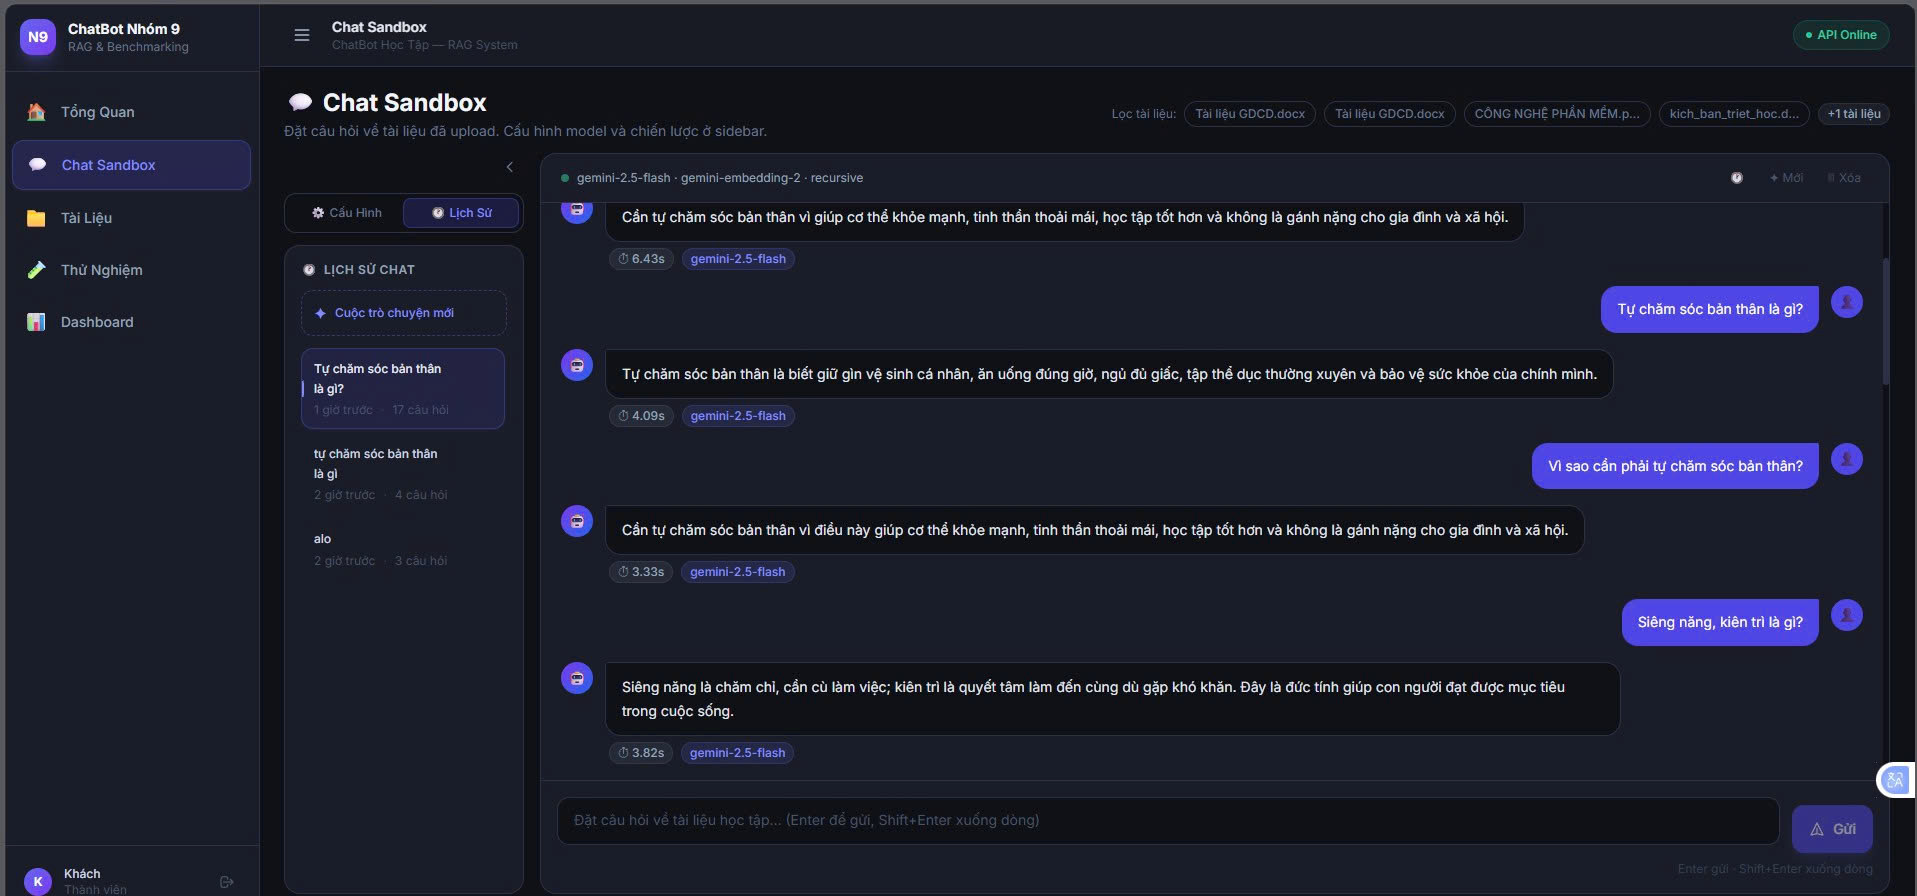
\includegraphics[width=\textwidth]{images/test_1.jpg}
  \caption{Giao diện Quản lý Tài liệu (Document Management)}
  \label{fig:document-management}
\end{figure}

\subsection{FR-04: Chức năng Chat Sandbox (Cấu hình RAG)}

\begin{funcbox}[FR-04 -- Chat Sandbox]
  \textbf{Trigger:} Người dùng truy cập trang Chat Sandbox và điều chỉnh cấu hình.\\[4pt]
  \textbf{Actor:} Sinh viên, Quản trị viên\\
  \textbf{Mục đích:} Cho phép người dùng thử nghiệm các cấu hình RAG khác nhau trong thời gian thực.\\[4pt]
  \textbf{Cấu hình có thể điều chỉnh:}
  \begin{itemize}[itemsep=2pt]
    \item \textbf{Top-K:} Số lượng đoạn tài liệu tối đa được truy xuất (mặc định: 5).
    \item \textbf{Embedding Model:} Google Gemini Embedding hoặc BAAI/bge-m3.
    \item \textbf{LLM Model:} Gemini 2.5 Flash (và các model khác nếu được cấu hình).
    \item \textbf{Chunking Strategy:} Recursive Character hoặc Fixed-size.
    \item \textbf{Tài liệu nguồn:} Chọn một hoặc nhiều tài liệu làm ngữ cảnh.
  \end{itemize}
\end{funcbox}

\begin{figure}[H]
  \centering
  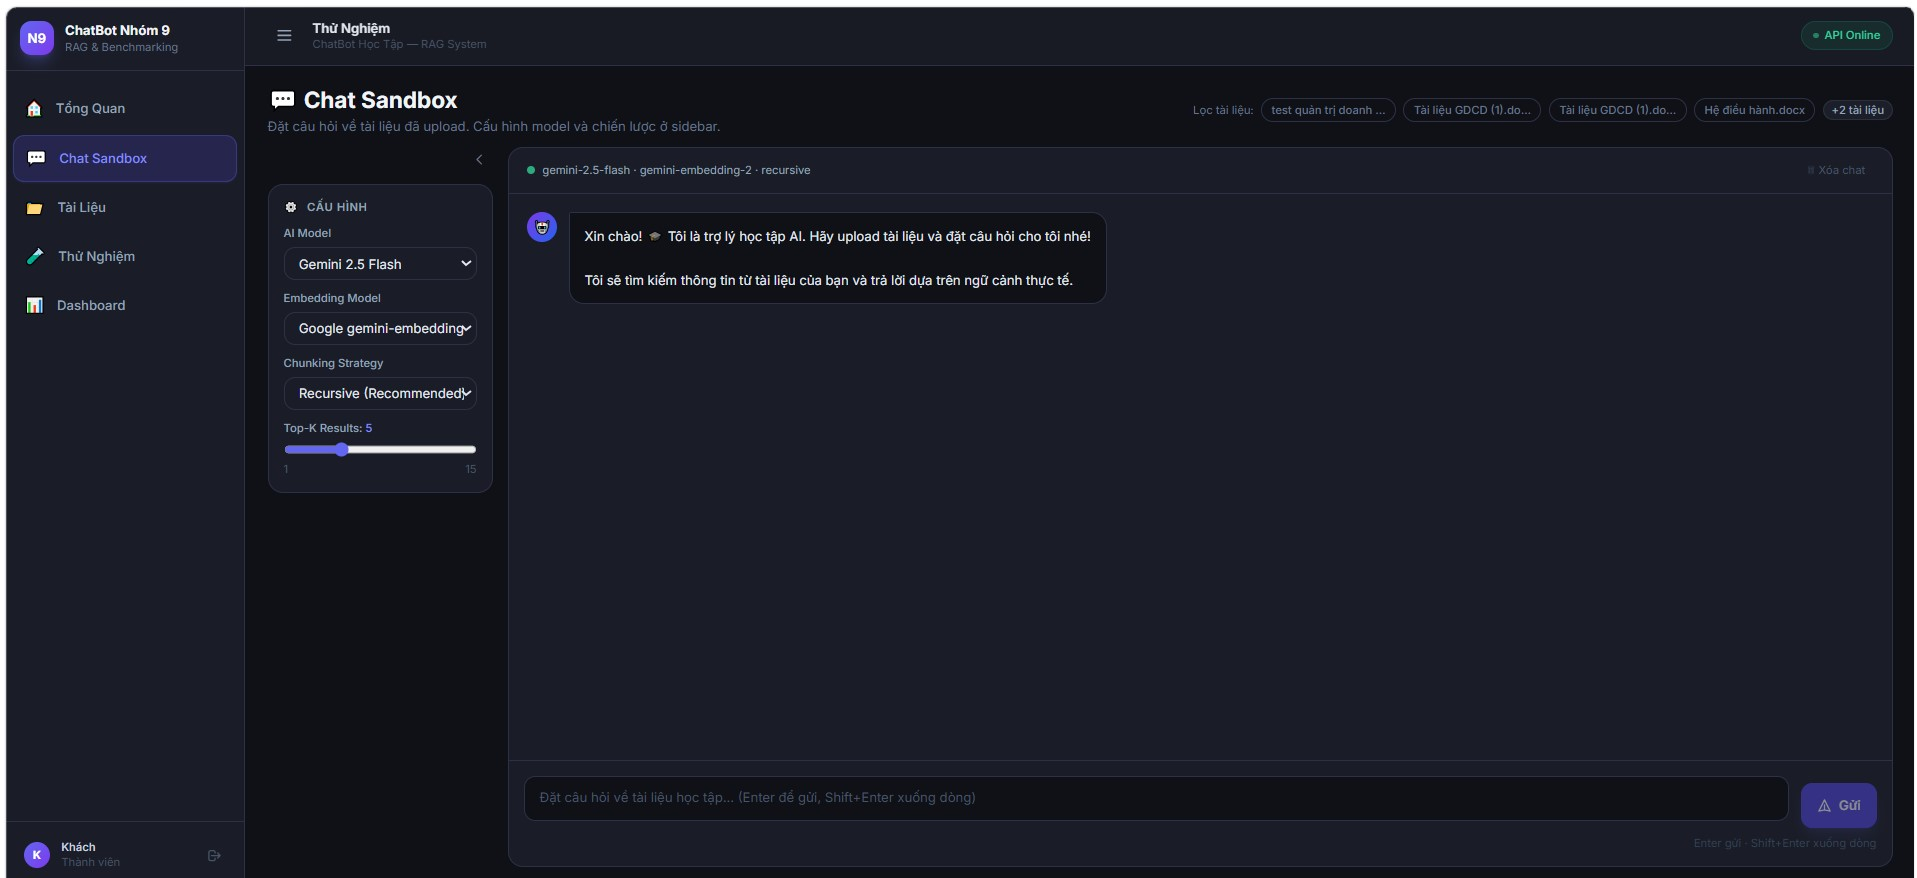
\includegraphics[width=\textwidth]{images/giao_dien_chat.jpg}
  \caption{Giao diện Chat Sandbox với bảng điều khiển cấu hình RAG}
  \label{fig:chat-sandbox}
\end{figure}

\subsection{FR-05: Chức năng Benchmark}

\begin{funcbox}[FR-05 -- Benchmark]
  \textbf{Trigger:} Quản trị viên cấu hình kịch bản và nhấn ``Chạy Benchmark''.\\[4pt]
  \textbf{Actor:} Quản trị viên\\
  \textbf{Mục đích:} Đánh giá định lượng chất lượng các cấu hình RAG khác nhau bằng bộ tiêu chí RAGAS.\\[4pt]
  \textbf{Luồng xử lý:}
  \begin{enumerate}[leftmargin=*, itemsep=2pt]
    \item Admin cấu hình kịch bản Benchmark: chọn cặp (Chunking Strategy, Embedding Model).
    \item Hệ thống nạp bộ câu hỏi kiểm thử (Test Dataset -- 50 câu hỏi).
    \item Với mỗi câu hỏi, hệ thống chạy toàn bộ chu trình RAG và ghi lại kết quả.
    \item Tính toán các chỉ số RAGAS: Accuracy, Relevancy, Faithfulness, Latency.
    \item Lưu kết quả vào MySQL và hiển thị lên Dashboard.
  \end{enumerate}
\end{funcbox}

\begin{figure}[H]
  \centering
  
\includegraphics[width=\textwidth]{images/test_benchmark.jpg}
  \caption{Giao diện cấu hình và chạy Benchmark}
  \label{fig:benchmark-ui}
\end{figure}

\subsection{FR-06: Chức năng Dashboard Phân tích}

\begin{funcbox}[FR-06 -- Dashboard Phân tích]
  \textbf{Trigger:} Người dùng truy cập trang Dashboard.\\[4pt]
  \textbf{Actor:} Quản trị viên\\
  \textbf{Mục đích:} Tổng hợp và trực quan hóa kết quả Benchmark qua biểu đồ Radar và bảng xếp hạng.\\[4pt]
  \textbf{Nội dung hiển thị:}
  \begin{itemize}[itemsep=2pt]
    \item Biểu đồ Radar so sánh các cấu hình RAG theo 4 chỉ số RAGAS.
    \item Bảng xếp hạng các cấu hình từ tốt đến kém.
    \item Biểu đồ xu hướng Latency theo từng kịch bản Benchmark.
    \item Tổng số tài liệu, tổng số câu hỏi đã hỏi, thời gian phản hồi trung bình.
  \end{itemize}
\end{funcbox}

\begin{figure}[H]
  \centering
  
\includegraphics[width=\textwidth]{images/dashboard.jpg}
  \caption{Dashboard tổng quan các chỉ số RAGAS}
  \label{fig:dashboard}
\end{figure}

\begin{figure}[H]
  \centering
  
\includegraphics[width=\textwidth]{images/dashboard1.jpg}
  \caption{Biểu đồ Radar và bảng xếp hạng các cấu hình RAG}
  \label{fig:radar}
\end{figure}

%------------------------------------------------------
\section{Yêu cầu Phi Chức năng (Non-Functional Requirements)}
%------------------------------------------------------

\subsection{Hiệu năng (Performance)}

\begin{itemize}[itemsep=4pt]
  \item \textbf{NFR-01:} Thời gian phản hồi (Latency) cho một câu hỏi thông thường \textless{} 5 giây.
  \item \textbf{NFR-02:} Thời gian xử lý Ingestion cho tài liệu 50 trang \textless{} 2 phút.
  \item \textbf{NFR-03:} Tốc độ truy vấn ChromaDB \textless{} 500ms cho tập dữ liệu $\leq$ 100,000 vectors.
  \item \textbf{NFR-04:} Hệ thống phải hỗ trợ ít nhất 10 người dùng đồng thời mà không suy giảm hiệu năng.
\end{itemize}

\subsection{Độ chính xác (Accuracy \& Faithfulness)}

\begin{itemize}[itemsep=4pt]
  \item \textbf{NFR-05:} Chỉ số Faithfulness (đo bằng RAGAS) phải đạt $\geq$ 0.85.
  \item \textbf{NFR-06:} Chỉ số Relevancy phải đạt $\geq$ 0.80.
  \item \textbf{NFR-07:} Hệ thống phải từ chối trả lời (thay vì hallucinate) khi không tìm thấy thông tin liên quan trong tài liệu.
\end{itemize}

\subsection{Bảo mật (Security)}

\begin{itemize}[itemsep=4pt]
  \item \textbf{NFR-08:} Phân quyền rõ ràng: chỉ Quản trị viên được phép xóa tài liệu và chạy Benchmark.
  \item \textbf{NFR-09:} API Key của LLM (Gemini) phải được lưu trong biến môi trường (.env), không hardcode trong mã nguồn.
  \item \textbf{NFR-10:} Dữ liệu người dùng phải được bảo vệ, không lưu thông tin nhạy cảm dạng plain text.
\end{itemize}

\subsection{Khả năng Mở rộng (Scalability)}

\begin{itemize}[itemsep=4pt]
  \item \textbf{NFR-11:} Kiến trúc phải cho phép dễ dàng thay thế/bổ sung mô hình LLM hoặc Embedding Model mà không cần sửa đổi logic nghiệp vụ cốt lõi (Interface Pattern).
  \item \textbf{NFR-12:} ChromaDB phải hỗ trợ tối thiểu 1,000 tài liệu (khoảng 10 triệu chunks) trong tương lai.
\end{itemize}

\subsection{Khả dụng (Availability)}

\begin{itemize}[itemsep=4pt]
  \item \textbf{NFR-13:} Backend FastAPI phải hỗ trợ xử lý bất đồng bộ (Async I/O) để phục vụ nhiều sinh viên cùng lúc.
  \item \textbf{NFR-14:} Hệ thống phải có cơ chế xử lý lỗi (Error Handling) và trả về thông báo lỗi rõ ràng khi API bên ngoài không phản hồi.
\end{itemize}

\subsection{Khả năng Bảo trì (Maintainability)}

\begin{itemize}[itemsep=4pt]
  \item \textbf{NFR-15:} Code phải tuân thủ chuẩn PEP 8 (Python) và ESLint Airbnb (JavaScript).
  \item \textbf{NFR-16:} Tài liệu API phải được sinh tự động bằng Swagger/OpenAPI.
  \item \textbf{NFR-17:} Module hóa rõ ràng: mỗi module (RAG, Benchmark, Auth) là một package độc lập.
\end{itemize}

%------------------------------------------------------
\section{Yêu cầu Giao diện Ngoài (External Interface Requirements)}
%------------------------------------------------------

\subsection{Giao diện Người dùng (User Interface)}

\begin{itemize}[itemsep=3pt]
  \item Giao diện Web hiển thị tốt trên các trình duyệt hiện đại (Chrome, Firefox, Edge).
  \item Thiết kế Responsive, hỗ trợ màn hình từ 1024px trở lên.
  \item Hỗ trợ Dark/Light mode (tùy chọn).
  \item Khu vực Chat phải có thanh cuộn (scroll) khi lịch sử dài.
\end{itemize}

\subsection{Giao diện Phần mềm (Software Interface)}

\begin{table}[H]
  \centering
  \caption{Danh sách giao diện phần mềm bên ngoài}
  \label{tab:sw-interfaces}
  \renewcommand{\arraystretch}{1.4}
  \begin{tabularx}{\textwidth}{|l|l|X|}
    \hline
    \rowcolor{blue!10}
    \textbf{Hệ thống} & \textbf{Giao thức} & \textbf{Mô tả} \\
    \hline
    Google Gemini API & HTTPS/REST & Gọi LLM để sinh câu trả lời và tạo Text Embedding. \\
    \hline
    BAAI/bge-m3 & Python Library & Embedding cục bộ không cần API key. \\
    \hline
    ChromaDB & Python SDK & Lưu trữ và truy vấn Vector Embedding nội bộ. \\
    \hline
    MySQL & SQLAlchemy ORM & Lưu trữ metadata, lịch sử chat, kết quả Benchmark. \\
    \hline
    PyPDF / pdfplumber & Python Library & Trích xuất văn bản từ file PDF. \\
    \hline
  \end{tabularx}
\end{table}

%------------------------------------------------------
\section{Phụ lục Yêu cầu (Requirements Appendix)}
%------------------------------------------------------

\subsection{Danh sách Thông báo Hệ thống (Application Messages List)}

\begin{table}[H]
  \centering
  \caption{Danh sách thông báo hệ thống}
  \label{tab:messages}
  \renewcommand{\arraystretch}{1.4}
  \begin{tabularx}{\textwidth}{|c|l|X|l|}
    \hline
    \rowcolor{blue!10}
    \textbf{Mã} & \textbf{Loại} & \textbf{Nội dung thông báo} & \textbf{Trigger} \\
    \hline
    MSG-01 & Thành công & ``Tài liệu đã được xử lý thành công và sẵn sàng sử dụng.'' & Ingestion hoàn tất. \\
    \hline
    MSG-02 & Lỗi & ``Định dạng file không được hỗ trợ. Chỉ chấp nhận PDF và DOCX.'' & Sai định dạng. \\
    \hline
    MSG-03 & Lỗi & ``Không tìm thấy thông tin liên quan trong kho tài liệu.'' & ChromaDB trả về rỗng. \\
    \hline
    MSG-04 & Cảnh báo & ``Kết nối tới LLM API bị gián đoạn. Vui lòng thử lại.'' & API timeout. \\
    \hline
    MSG-05 & Thông tin & ``Benchmark đang chạy. Vui lòng chờ...'' & Benchmark bắt đầu. \\
    \hline
    MSG-06 & Thành công & ``Benchmark hoàn tất. Xem kết quả tại Dashboard.'' & Benchmark xong. \\
    \hline
    MSG-07 & Lỗi & ``Kích thước file vượt quá giới hạn cho phép (50MB).'' & File quá lớn. \\
    \hline
  \end{tabularx}
\end{table}

\subsection{Thuật ngữ Giải thích (Glossary)}

\begin{table}[H]
  \centering
  \caption{Bảng thuật ngữ sử dụng trong tài liệu}
  \label{tab:glossary}
  \renewcommand{\arraystretch}{1.4}
  \begin{tabularx}{\textwidth}{|l|X|}
    \hline
    \rowcolor{blue!10}
    \textbf{Thuật ngữ} & \textbf{Định nghĩa} \\
    \hline
    RAG & Retrieval-Augmented Generation -- Kỹ thuật kết hợp truy xuất tài liệu với sinh ngôn ngữ. \\
    \hline
    LLM & Large Language Model -- Mô hình ngôn ngữ lớn (ví dụ: Gemini, GPT). \\
    \hline
    Embedding & Biểu diễn văn bản dưới dạng vector đa chiều. \\
    \hline
    Chunking & Kỹ thuật phân mảnh văn bản thành các đoạn nhỏ hơn. \\
    \hline
    Hallucination & Hiện tượng AI tự bịa đặt thông tin không có trong dữ liệu huấn luyện. \\
    \hline
    RAGAS & Retrieval Augmented Generation Assessment -- Bộ tiêu chí đánh giá hệ thống RAG. \\
    \hline
    Top-K & Số lượng đoạn tài liệu liên quan nhất được truy xuất từ ChromaDB. \\
    \hline
    Ingestion Pipeline & Luồng xử lý tự động từ lúc tải file đến khi lưu vào ChromaDB. \\
    \hline
    Cosine Similarity & Phép đo độ tương đồng giữa hai vector bằng cách đo góc giữa chúng. \\
    \hline
  \end{tabularx}
\end{table}

\section{Kết luận Chương}

Chương này đã trình bày đầy đủ đặc tả yêu cầu phần mềm (SWR) của hệ thống Chatbot RAG, bao gồm: biểu đồ ngữ cảnh, biểu đồ Use Case tổng quan, đặc tả chi tiết 6 nhóm chức năng chính (với Function Trigger, luồng xử lý và Business Rules), các yêu cầu phi chức năng về hiệu năng/bảo mật/khả năng mở rộng, và phụ lục danh sách thông báo hệ thống. Đây là nền tảng kỹ thuật quan trọng để thiết kế kiến trúc chi tiết trong chương SWD tiếp theo.
